% siminos/atlas/slice.tex  pdflatex atlas
% $Author$ $Date$


\section{Reduction of continuous symmetry}
\label{s:slice}

%%%%%%%%%%%%%%%%%%%%%%%%%%%%%%%%%%%%%%%%%%%%%%%%%
% 2011-08-23 Predrag: replaces BeThTraj.pdf from
% dasbuch/book/FigSrc/inkscape/BeThTraj.svg
% 2011-09-09 Predrag: updated
%            continuous.tex overheads, and ChaosBook
\begin{figure}
 \begin{center}
  \setlength{\unitlength}{0.20\textwidth}
  %% \unitlength = units used in the Picture Environment
(a)~~
  \begin{picture}(1,1.07471658)%
    \put(0,0){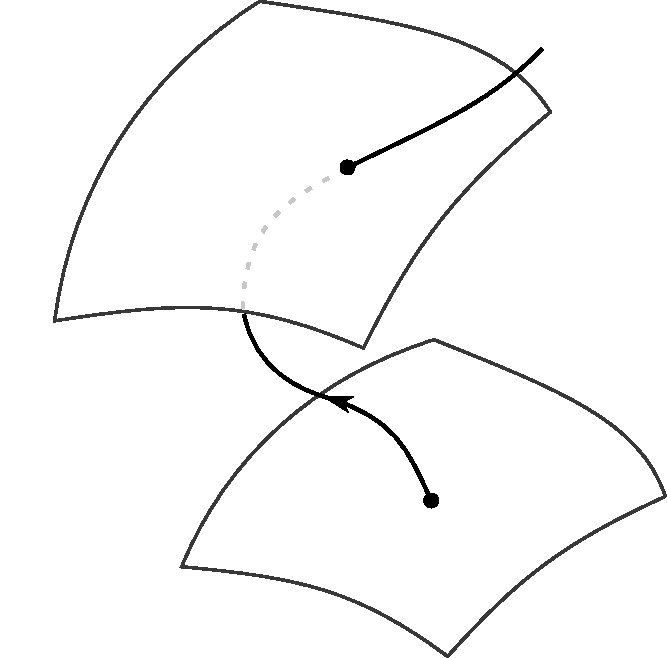
\includegraphics[width=\unitlength]{BeThTrajTeX}}%
    \put(0.28879298,1.02196543){\color[rgb]{0,0,0}\rotatebox{-22.37140782}{\makebox(0,0)[lb]{\smash{$\pS_{\ssp(\zeit)}$}}}}%
    \put(0.55566402,0.45078735){\color[rgb]{0,0,0}\rotatebox{-16.6673442}{\makebox(0,0)[lb]{\smash{$\pS_{\ssp(0)}$}}}}%
    \put(0.63028127,0.18433597){\color[rgb]{0,0,0}\rotatebox{0.03136739}{\makebox(0,0)[lb]{\smash{$\ssp(0)$}}}}%
    \put(0.46253394,0.70182304){\color[rgb]{0,0,0}\rotatebox{0.03136739}{\makebox(0,0)[lb]{\smash{$\ssp(\zeit)$}}}}%
    \put(0.03852492,0.09250899){\color[rgb]{0,0,0}\rotatebox{0.11031334}{\makebox(0,0)[lb]{\smash{$\pS$}}}}%
  \end{picture}%
~~(b)
  \begin{picture}(1,1.07315413)%
    \put(0,0){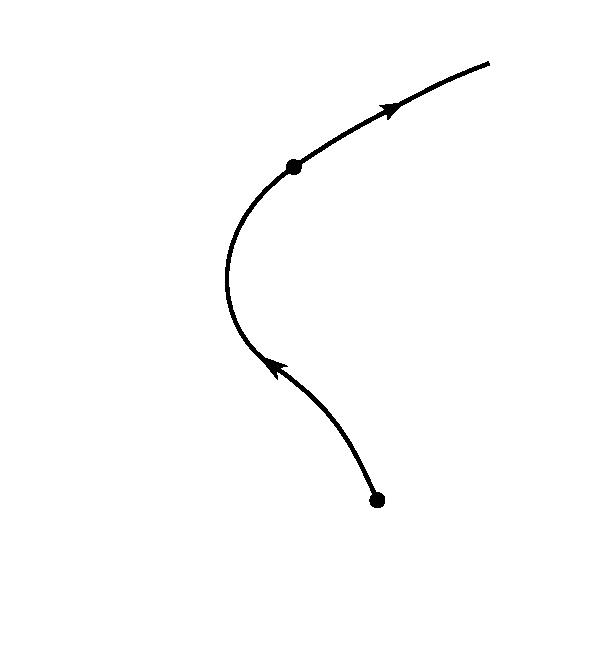
\includegraphics[width=\unitlength]{BeThRedTeX}}%
    \put(0.19912369,0.17144733){\color[rgb]{0,0,0}\rotatebox{0.11031334}{\makebox(0,0)[lb]{\smash{$\pSRed$}}}}%
    \put(0.63028127,0.18433598){\color[rgb]{0,0,0}\rotatebox{0.03136739}{\makebox(0,0)[lb]{\smash{$\sspRed(0)$}}}}%
    \put(0.46253394,0.70182305){\color[rgb]{0,0,0}\rotatebox{0.03136739}{\makebox(0,0)[lb]{\smash{$\sspRed(\zeit)$}}}}%
  \end{picture}%
 \end{center}
% (a) 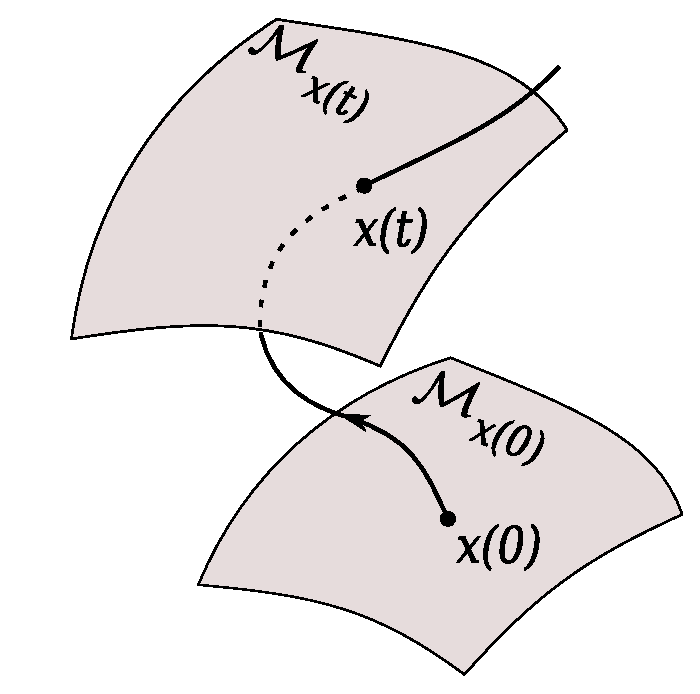
\includegraphics[width=0.45\textwidth]{BeThTraj}
  \caption{\label{fig:BeThTraj}
(a)
The group orbit $\pS_{\ssp(0)}$ of \statesp\ point $\ssp(0)$, and the
group orbit $\pS_{\ssp(\zeit)}$ reached by the trajectory $\ssp(\zeit)$ time $t$
later.
(b)
Symmetry reduction $\pS \to \pSRed$ replaces each full \statesp\
group orbit $\pS_{\ssp}\subset\pS$ by a single point $\sspRed \in \pSRed$.
  }
\end{figure}
%%%%%%%%%%%%%%%%%%%%%%%%%%%%%%%%%%%%%%%%%%%%%%%%%%

    \DB{2012-03-28}{
    at this point the writing abruptly jumps from goody-goody intro for
    the everyman to technical without sufficient warning. Need to segway
    into the group theory stuff
    }
This problem is here resolved by the
{\mslices}\rf{rowley_reconstruction_2000,BeTh04,SiCvi10,FrCv11}, in which
the group orbit of any full-flow structure is represented by a single
point (see \reffig{fig:BeThTraj}), the group orbit's intersection with a
fixed hypersurface, or the \emph{`\slice'}. A \slice\ fixes only the
symmetry group phases: a continuous time full space orbit is reduced to a
continuous time orbit in the symmetry-\reducedsp, as in
\reffig{f:MeanVelocityFrame}.


In the \mslices\ the symmetry reduction is achieved by cutting the group
orbits with a finite set of hyperplanes, one for each continuous group
parameter, with each group orbit of symmetry-equivalent points
represented by a single point, its intersection with the \slice. The
procedure is akin to (but distinct from) cutting across continuous-time
parametrized trajectories by means of Poincar\'e sections. A \PoincSec\
reduces a continuous time orbit to a sequence of points. \Slice, however,
is emphatically \emph{not} a \PoincSec; it replaces a continuous time
orbit ba a symmetry-reduced continuous time orbit.
    \PC{replace the term `symmetry reduction' by a term that does not
    (1) does not imply `reduction' (2) does not conflict with Lie theory
    and gen. relativity meaning of the term
    }

What follows is very much like the the \refsect{s:cut}; due to the linear
action of the symmetry group, 'slicing' is easier that `sectioning', but
more unfamiliar - that is why we started with reviewing Poincar\'e
sections.

\subsection{The 3 ideas}

\subsection{The 3 bridges to nowhere}

Purely group-theoretical, no dynamics to inform it.

\subsubsection{Polar coordinates}

\subsubsection{Hilbert bases}

\DB{2012-04-10}{A book report on Hilbert bases by Daniel Borrero}
One approach to symmetry reduction that is often used for low-dimensional
dynamical systems is to rewrite the dynamics in terms of a Hilbert
invariant polynomial basis (see \refref{GL-Gil07b} for a clear and
detailed discussion of this method). The idea here is that one can take
the dynamics in equivariant state space coordinates
$(x_1,x_2,x_3,...,x_d)$ and rewrite them in terms of polynomials of these
variables $(u_1,u_2,u_3,...,u_m)$ that are invariant under the group
action. In general, these polynomials are non-unique and $m \geq d$, so
that the flow becomes embedded in a larger m-dimensional state space.
While these polynomials are linearly independent, they are functionally
dependent by a set of relations called syzygies. The syzygies constrain
the flow to lower dimensional, but non-trivial, manifolds in the
m-dimensional space. They also introduce singularities in the flow, which
must be dealt with carefully.

Sometimes the determination of a Hilbert basis can be informed by
intuition about nonlinear preserved quantities such as rotationally
invariant length $r^2 = x_1^2 + x_2^2 + ... + x_d^2$. In general,
however, there is no general strategy for creating a useful Hilbert
basis. The algebra required is quite involved and the required
computations become very large for problems with as few as ten
dimensions\rf{gatermannHab}. This makes the method of Hilbert bases
unfeasible for dealing with turbulent fluid flows.

\subsubsection{Method of connections}

%%%%%%%%%%%%%%%%%%%%%%%%%%%%%%%%%%%%%%%%%%%%%%%%%%%%%%%%%%%%%%%%%%%%%
\begin{figure}
   \centering
  \setlength{\unitlength}{0.20\textwidth}
(a)~~~
  \begin{picture}(1,0.98073806)%
    \put(0,0){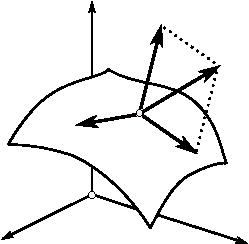
\includegraphics[width=\unitlength]{A28tangents}}%
    \put(0.8635648,0.73622308){\color[rgb]{0,0,0}\makebox(0,0)[lb]{\smash{$\vel$}}}%
    \put(0.49893205,0.86039365){\color[rgb]{0,0,0}\makebox(0,0)[lb]{\smash{$\vel_{\bot}$}}}%
    \put(0.27198728,0.5378933){\color[rgb]{0,0,0}\makebox(0,0)[lb]{\smash{$\groupTan_1$}}}%
    \put(0.58493215,0.33483773){\color[rgb]{0,0,0}\makebox(0,0)[lb]{\smash{$\groupTan_2$}}}%
    \put(0.54959234,0.21257862){\color[rgb]{0,0,0}\makebox(0,0)[lb]{\smash{$\LieEl\ssp$}}}%
  \end{picture}%
(b)~~~
  \begin{picture}(1,0.98655417)%
    \put(0,0){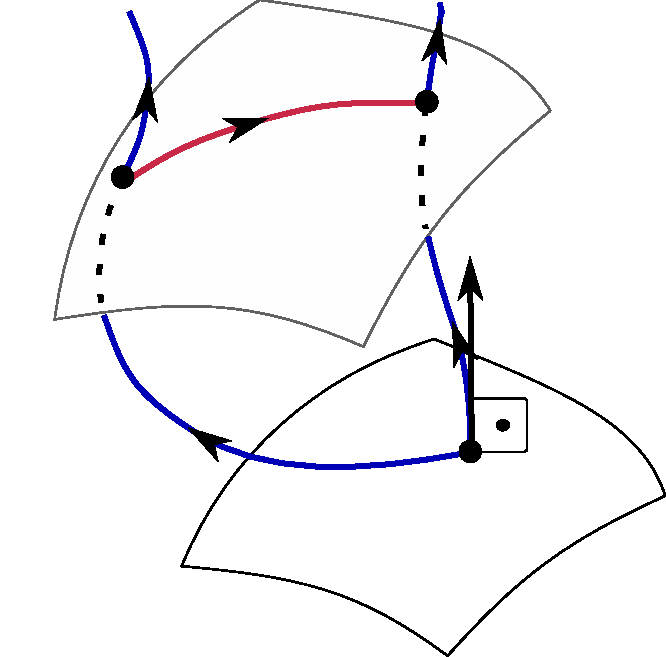
\includegraphics[width=\unitlength]{BeThMconnect}}%
    \put(0.20559239,0.64023845){\color[rgb]{0,0,0}\rotatebox{0.0313674}{\makebox(0,0)[lb]{\smash{$\ssp(\zeit)$}}}}%
    \put(0.68383186,0.20519203){\color[rgb]{0,0,0}\rotatebox{0.0313674}{\makebox(0,0)[lb]{\smash{$\ssp(0)$}}}}%
    \put(0.67475925,0.8109461){\color[rgb]{0,0,0}\rotatebox{0.0313674}{\makebox(0,0)[lb]{\smash{$\sspRed(\zeit)$}}}}%
    \put(0.35760559,0.8662057){\color[rgb]{0,0,0}\rotatebox{0.0313674}{\makebox(0,0)[lb]{\smash{$\LieEl(\zeit)$}}}}%
    \put(0.70884327,0.61850672){\color[rgb]{0,0,0}\rotatebox{0.0313674}{\makebox(0,0)[lb]{\smash{$\vel_{\bot}$}}}}%
  \end{picture}%
   \caption{\label{fig:BeThMconnect}
    (a)
By equivariance $\vel(\ssp)$ can be replaced by $\vel_\bot(\ssp)$, the
velocity normal to the group tangent directions at \statesp\ point $\ssp$.
    (b)
``Method of connections'' replaces $\vel(\sspRed)$ at every instant
$\sspRed =\sspRed(\zeit)$ by the velocity $\vel_\bot(\sspRed)$, so in
$\sspRed(\zeit)$ co-moving frame there is no motion along the group
tangent directions.
}
\end{figure}
%%%%%%%%%%%%%%%%%%%%%%%%%%%%%%%%%%%%%%%%%%%%%%%%%%%%%%%%%%%%%%%%%%%%%

 \mslices

    \begin{itemize}
      \item closest point on a group orbit
      \item variation $\to$ \slice\ hyperplane
    \end{itemize}

\subsection{The goal, 3 ideas}

The goal of \emph{symmetry reduction} is to replace each group orbit by a
unique point in a lower-dimensional symmetry-\reducedsp\ $\pSRed =
\pS/\Group$, as sketched in \reffig{fig:BeThTraj}.


... the same templates as those used in \refsect{s:cut} to define local
sections of time trajectories...

\subsection{\Mslices; a local chart}

This paper has two ideas:
\begin{enumerate}
  \item slice locally
  \item chart globally
\end{enumerate}


Symmetries of the flow (i.e.\ the transformations $\LieEl\in\Group$) are
then used to shift and rotate the {\template} $\slicep$ until it
overlies, as well as possible, the state $\ssp$, by minimizing the
distance
\beq
\Norm{\ssp - \LieEl(\gSpace)\,\slicep}
\, .
\ee{minDistance}
The entire group orbit of $\ssp$ is then replaced by the closest match to
the template pattern, given by $\sspRed=\LieEl^{-1}\ssp$. The
symmetry-\reducedsp\ $\pSRed$ (hereafter referred to as the `slice'), of
dimension $(d\!-\!1)$, consists of the set of closest matches $\sspRed$,
one element for each full \statesp\ $\pS$ group orbit; the hat on
$\sspRed$ indicates the unique point on the group orbit of $\ssp$ closest
to the \template\ \slicep.

%%%%%%%%%%%%%%%%%%%%%%%%%%%%%%%%%%%%%%%%%%%%%%%%%%%%%%%%%%%%%%%%%%%%%
\begin{figure}
   \centering
(b)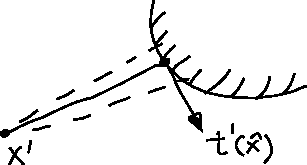
\includegraphics[width=0.20\textwidth]{A28extremum}
   \caption{\label{fig:A28extremum}
    (b)
Extremal condition for nearest distance.
}
\end{figure}
%%%%%%%%%%%%%%%%%%%%%%%%%%%%%%%%%%%%%%%%%%%%%%%%%%%%%%%%%%%%%%%%%%%%%


For the reduction of a $\SOn{2}$ symmetry, the minimal distance satisfies
the extremum condition
    \PC{make 2 lines?}
\[
\frac{\partial}{\partial \gSpace} \Norm{\ssp - \LieEl(\gSpace)\,\slicep}^2
   =
2\, \braket{\sspRed - \slicep}{\sliceTan{}}
   = 0
        \,,\quad
\sliceTan{} = \Lg \slicep
\,.
\]
$\Norm{\LieEl(\gSpace)\slicep}$ is a constant, the group tangent vector
$\sliceTan{}$ evaluated at $\slicep$ \refeq{eq:tang} is normal to
$\slicep$, and the term $\braket{\slicep}{\Lg \,\slicep}$ vanishes ($\Lg$
is antisymmetric). Therefore  $\sspRed$, the point on the group orbit that
lands in the \slice, satisfies the \emph{\slice\ condition}
\beq
\braket{\sspRed}{\sliceTan{}} = 0
    \,.
\ee{PCsectQ0}
The \slice\ so defined is thus a hyperplane
normal to the \template\ group tangent evaluated at the \template.
As the symmetries do not act on the invariant subspaces, for them
$\sliceTan{} = 0$, and they are contained within all slices.

Conversely,
a template has to be equivariant under infinitesimal actions of the symmetry
group in order that the slice is of dimensionality $(d-N)$.
In the choice of the {\template} one should avoid solutions
that belong to the invariant or partially symmetric subspaces; for such
choices $\Lg_{a}\slicep=0$, and some or all $\sliceTan{a}$ vanish identically
and impose no slice conditions. The {\template} $\slicep$ should be a
generic \statesp\ point in the sense that its group orbit has the full
$N$ dimensions of the group \Group.
The set of the group orbit points \emph{closest} to the \template\ \slicep\
form an open connected neighborhood
of \slicep, a neighborhood in which each group orbit intersects the
hyperplane \emph{only once}.
This neighborhood is contained in
a half-hyperplane, bounded on one side by the intersection of the hyperplane section
with its {\chartBord}.

In what follows we shall refer to this connected open neighborhood
of \slicep\ as a \emph{\slice} $\pSRed_{\slicep} \supset \pS/\Group$,
and
to  \refeq{??PCsectQ} as the \emph{slice conditions}.

%%%%%%%%%%%%%%%%%%%%%%%%%%%%%%%%%%%%%%%%%%%%%%%%%%%%%%%%%%%%%%%%
%% slice.*, inflectHype.*: see dasbuch/book/FigSrc/inkscape/00ReadMe.txt
%% rpo.* hand-drawn in dasbuch/book/FigSrc/xfig/rpo.fig
%% xfig exported -> FigSrc/inkscape/rpo.fig
%% inkscape exported -> rpo.eps + LaTeX, hand edited in the macros
%% Predrag 2011-08-27 replaced rpo.pdf by rpoSlice.pdf
%% remember to insert rpoSlice.pdf into ChaosBook

 \begin{figure}
 \begin{center}
  \setlength{\unitlength}{0.40\textwidth}
  %% \unitlength = units used in the Picture Environment
(a)
  \begin{picture}(1,0.87085079)%
    \put(0,0){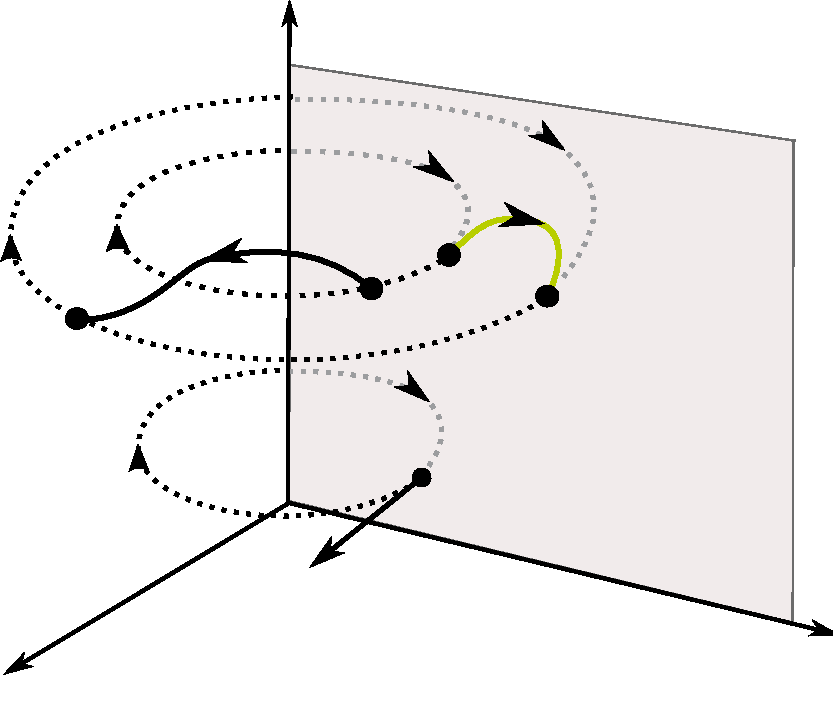
\includegraphics[width=\unitlength]{slice}}%
    \put(0.82835155,0.19007659){\color[rgb]{0,0,0}\rotatebox{-14.84025424}{\makebox(0,0)[lb]{\smash{$\pSRed$}}}}%
    \put(0.07077338,0.28688228){\color[rgb]{0,0,0}\rotatebox{0.0313674}{\makebox(0,0)[lb]{\smash{$\LieEl\,\slicep$}}}}%
    \put(0.53023327,0.26593335){\color[rgb]{0,0,0}\rotatebox{0.0313674}{\makebox(0,0)[lb]{\smash{$\slicep$}}}}%
    \put(0.4284954,0.179285){\color[rgb]{0,0,0}\rotatebox{0.0313674}{\makebox(0,0)[lb]{\smash{$\sliceTan{}$}}}}%
    \put(0.00798985,0.42305068){\color[rgb]{0,0,0}\rotatebox{0.0313674}{\makebox(0,0)[lb]{\smash{$\ssp(\zeit)$}}}}%
    \put(0.65766235,0.45412105){\color[rgb]{0,0,0}\rotatebox{0.0313674}{\makebox(0,0)[lb]{\smash{$\sspRed(\zeit)$}}}}%
    \put(0.06916446,0.74280851){\color[rgb]{0,0,0}\rotatebox{0.0313674}{\makebox(0,0)[lb]{\smash{$\LieEl(\zeit)$}}}}%
  \end{picture}%
\\ %~~~
(b)
  \begin{picture}(1,0.87085079)%
    \put(0,0){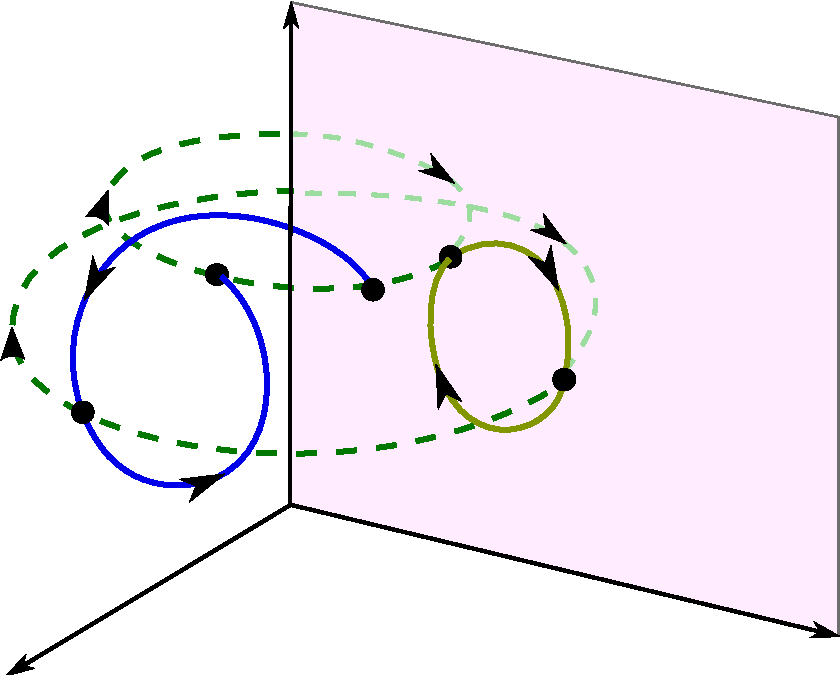
\includegraphics[width=\unitlength]{rpoSlice}}%
    \put(0.82835153,0.19007656){\color[rgb]{0,0,0}\rotatebox{-14.84025432}{\makebox(0,0)[lb]{$\pSRed$}}}%
    \put(0.40925459,0.45713857){\color[rgb]{0,0,0}\rotatebox{0.0313674}{\makebox(0,0)[lb]{\smash{$\ssp(0)$}}}}%
    \put(0.71354118,0.39765314){\color[rgb]{0,0,0}\rotatebox{0.0313674}{\makebox(0,0)[lb]{\smash{$\sspRed(\zeit)$}}}}%
    \put(0.13171187,0.38813817){\color[rgb]{0,0,0}\rotatebox{0.0313674}{\makebox(0,0)[lb]{\smash{$\LieEl(\zeit)$}}}}%
    \put(0.02168739,0.31359574){\color[rgb]{0,0,0}\rotatebox{0.0313674}{\makebox(0,0)[lb]{\smash{$\ssp(\zeit)$}}}}%
    \put(0.15576193,0.48769256){\color[rgb]{0,0,0}\rotatebox{0.0313674}{\makebox(0,0)[lb]{\smash{$\ssp(\period{})$}}}}%
    \put(0.54113911,0.50476963){\color[rgb]{0,0,0}\rotatebox{0.0313674}{\makebox(0,0)[lb]{\smash{$\sspRed(0)$}}}}%
  \end{picture}%
 \end{center}
 \caption{\label{fig:slice}
The \mslices, a \statesp\ visualization:
(a)
\Slice\ $\pSRed \supset \pS/\Group$ lies in the $(d\!-\!N)$\dmn\
hyperplane \refeq{PCsectQ0} normal to $\sliceTan{}$, where $\sliceTan{j}$
span the  $N$\dmn\ space tangent to the group orbit $\LieEl\,\slicep$
(dotted line) evaluated at the {\template} point $\slicep$. The
hyperplane intersects {all} full \statesp\ group orbits (green
dashes).  This is a highly idealized sketch: A group orbit is a $N$\dmn\
manifold, and even for $\SOn{2}$ it is usually only topologically a
circle (see \reffig{fig:2840GOt135th0}), and can intersect a hyperplane
any number of times  (see \reffig{fig:sliceimage}). The full \statesp\
trajectory $\ssp(\zeit)$ (blue) and the \reducedsp\ trajectory
$\sspRed(\zeit)$ (green) are equivalent up to a `moving frame' rotation
$\ssp(\zeit)=\LieEl(\zeit)\,\sspRed(\zeit)$, where $\LieEl(\zeit)$ is a
shorthand for $\LieEl(\gSpace(\zeit))$.
(b)
In the full \statesp\ $\pS$ a \rpo\ $\ssp(0) \to \ssp(\zeit) \to
\ssp(\period{})$ returns to the group orbit of $\ssp(0)$ after time
$\period{}$ and a rotation by $\LieEl$,  $\ssp(0)=\LieEl \, \ssp
(\period{})$. A generic \rpo\ fills out quasi-\-periodically what is
topologically a torus (\reffig{fig:CLf01group}). In the \slice\ $\pSRed$
the symmetry-reduced orbit is periodic, $\sspRed(0) =
\sspRed(\period{})$.
 }
 \end{figure}


When $\ssp$ is varies in time, $\dot{\ssp}=\vel(\ssp)$, the {\template}
$\slicep$ tracks the motion using the slice condition \refeq{PCsectQ0} to
minimize $\Norm{\ssp(\zeit)-\LieEl(\theta(\zeit))\slicep}$, and the
full-space trajectory $\ssp(\zeit)$ is thus rotated into the
{\reducedsp}, $\sspRed(\zeit) = \LieEl^{-1}\,\ssp(\zeit)$, by appropriate
\emph{moving frame} angles $\{\gSpace(\zeit)\}$, as depicted in
\reffig{fig:slice}\,{(a)}. Specializing to $\SOn{2}$, one can write
the equations for the \reducedsp\ flow, $\dot{\sspRed} =
\velRed(\sspRed)$, confined to the \slice, $\sspRed(\zeit) \in \pSRed$,
as
\bea
\velRed(\sspRed) &=& \vel(\sspRed)
     \,-\, \dot{\gSpace}(\sspRed) \, \groupTan(\sspRed)
\label{EqMotMFrame}\\
\dot{\gSpace}(\sspRed) &=& \braket{\vel(\sspRed)}{\sliceTan{}}
                       /\braket{\groupTan(\sspRed)}{\sliceTan{}}
\,.
\label{reconstrEq}
\eea
In other words, $\vel$, the velocity in the full \statesp, can be written
as the sum of $\velRed$, the velocity component in the \slice, and
$\dot{\gSpace}\,\groupTan$, the Cartan derivative \refeq{CartanDer} or
the velocity component within the group tangent space. The
$\dot{\gSpace}$ equation is called the {\em reconstruction equation}, as its
integral keeps track of the group shift in the full \statesp. In
particular, if  \sspRed\ is a point on a \reqv\ \refeq{phaseVel}, the full \statesp\
velocity equals the phase velocity, and $\velRed(\sspRed) = 0$, \ie,
\reqva\ are always reduced to \eqva\ in the \reducedsp.

    \ifdraft\color{blue}
\subsection{What it is not}
    \begin{itemize}
      \item co-moving frame
      \item an average over the group phase variables?
        {\bf PC 2011-10-18} Note also that the rotation of a fluid flow
        into a \slice\ {\em is not} an average over the 3D pipe azimuthal
        angle, it is the full snapshot of the flow embedded in the
        $\infty$-dimensional \statesp. Symmetry reduction is not a
        dimensional-reduction scheme, or flow modeling by fewer degrees
        of freedom: it is a local change of coordinate, with one (or $N$)
        coordinates pointing along the phase direction. The \reducedsp\
        is also $\infty$-dimensional and no information is lost, one can
        go freely between solutions in the full and reduced \statesp s by
        integrating the associated \emph{reconstruction equations}.
      \item reduced-dimensionality model
      \item {\bf DB 2012-03-27} It is not the ``embedded template'' used in the topological theory of
      low dimensional chaos. In Predrag's words, ``It is not THAT template''.
    \end{itemize}
    \color{black}\fi
